\chapter{Extensibility and Multi-Tenancy}
Today's model of separated compute and storage is reaching its limits.  Fast,
  kernel-bypass networking has yielded key-value stores that perform
  millions of requests per second per machine with microseconds of
  latency~\cite{farm-2014,fasst-2016,mica,ramcloud,drtm}.
These systems gain much of their speed by being simple, allowing only lookups
  and updates.
However, this simplicity results in inefficient data movement between storage and
  compute and costly client-side stalls~\cite{killer-microseconds,grappa}.
To efficiently exploit these new stores, applications will be under
  increasing pressure to push compute to them, but the granularity at which
  they can do so is a concern.
At microsecond timescales, even small costs for isolation, containerization, or
  request dispatching dominate, placing practical limits on the granularity of
  functions that applications can offload to storage
  (Figure~\ref{fig:context-switches}).

\begin{figure}[t]
\centering
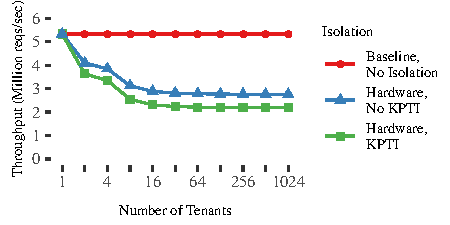
\includegraphics[width=1.0\columnwidth]{graphs/simulator.pdf}
\caption{Simulated throughput versus the number of tenants. With
	hardware isolation, even modestly increasing the number of
  tenants to 16 (just twice the number
	of cores) leads to a significant drop in throughput.
  ``No isolation'' represents an upper bound where isolation costs are zero.}
\label{fig:simulator}
\end{figure}


This tension is resolved in \textsl{Splinter}, a multi-tenant in-memory key-value store with
  a new approach to pushing compute to storage servers.
Splinter preserves the low remote access latency (9~\us) and high throughput (3.5~Mops/s)
  of in-memory storage
  while adding native-code runtime \textsl{extensions} and the dense
  \textsl{multi-tenancy} (thousands of tenants) needed in modern data centers.
Tenants send arbitrary type- and memory-safe extension code to
  stores at runtime, adding new operations, data types, or
  storage personalities.
These extensions are exposed so tenants can remotely
  invoke them to perform operations on
  their data.
Splinter's lightweight isolation lets thousands of untrusted tenants
  safely share storage and compute, giving them access to as
  much or as little storage as they need.

Splinter's design springs from the intersection of three trends:
  \textsl{in-memory storage with low-latency networking}, which is driving down
  the practical limits of request granularity;
\textsl{massive multi-tenancy} driven by the cloud and the efficiency gains of
  consolidation;
and \textsl{serverless computing}, which is already training developers to
  write stateless, decomposed application logic that can run anywhere in order to gain agility,
  scalability, and ease of provisioning.

Together, these trends drive Splinter's key design goals:
\begin{description}
\item[No-cost Isolation.]
  Since extensions come from untrusted tenants, they must be isolated from one
    another.
  Hardware-based isolation is too
    expensive at microsecond time scales; even a simple page table switch would
    significantly impact response time and throughput.
%  To solve this, Splinter enables developers to write type-safe, memory-safe
%    extensions in Rust~\cite{rust-2018}, avoiding hardware isolation costs.

\item[Zero-copy Storage Interface.]
  Extensions interact with stored data through a well-defined interface that
    serves as a trust boundary.
  For fine-grained requests, it
    must be lightweight in terms of transfer of control and in terms of
    data movement.
  This effectively requires extensions to be able to directly operate on tenant
    data \textit{in situ} in the store, while maintaining protection and
    preventing data races with each other and the storage engine.
%  Splinter's extension interface makes use of Rust's memory safety to pass
%    references to data objects across trust boundaries without any intervening
%    copies, while ensuring that untrusted code cannot access memory belonging
%    to other tenants.
%  Extensions can typecast these objects into a set of safe
%    types to achieve a rich data model without serialization and de-serialization costs.

\item[Lightweight Scheduling for Heterogeneous Tasks.]
  Extensions are likely to be heterogeneous.
  Some extensions might involve simple point lookups of data or constructing
    small indexes; others might involve expensive computation or more data.
  Preemptive scheduling involves costly context switches, so Splinter
    must avoid preemption in the normal case, yet maintain it as an option
    to contain poorly-behaving extensions.
  It must also be able to support high quality of service under heavy skew, 
    both in terms of the tenants issuing requests at different rates and
    extensions that take different amounts of time to complete.
%  primarily
%    relies on cooperative scheduling, expecting extensions to regularly yield
%    voluntarily.
%  Splinter borrows recent ideas in low-latency scheduling~\cite{arachne-2018}
%    and adapts them for untrusted code.
%  It reserves preemption for extensions that do not cooperate: it preempts them
%    to avoid starving other tenants, and the costs of preemption are paid only
%    by the misbehaving extension, preserving good quality of service for the
%    others.

\item[Adaptive Multi-core Request Routing.]
  With multiple tenants sharing a single machine, synchronization over tenant
    state can become a bottleneck.
  To minimize contention, tenants maintain locality by routing requests to
    preferred cores on Splinter servers.
  We can't, however, use a hard partitioning, as we don't want high skew to
    create hotspots and underused cores~\cite{zygos}.
    Routing decisions can't get in the way of fast dispatch of requests~\cite{ix}.
 % To prevent cores from becoming overloaded under high skew, Splinter uses
 %   \textit{work stealing}, allowing underloaded cores to steal requests from
 %   overloaded ones.

\end{description}

These goals give rise to Splinter's design.
Developers write type-safe, memory-safe extensions in Rust~\cite{rust}
that they push to Splinter servers.
Exploiting type-safety for lightweight isolation isn't new;
SPIN~\cite{spin} allowed applications to safely and dynamically load
extensions into its kernel by relying on language-enforced isolation.
Similarly, NetBricks~\cite{netbricks-2016} applied Rust's safety
properties to dataplane packet processing to
  provide memory safety between sets of compile-time-known domains comprising
  network function chains.
Splinter combines these approaches and applies them in a new and challenging domain.
Language-enforced isolation with native performance and without garbage
  collection overheads is well-suited to low-latency data-intensive services
  like in-memory stores --- particularly, when functionality must be added and removed at
  runtime by large numbers of fine-grained protection domains.

Splinter's approach allows it to scale to support thousands of tenants per
  machine, while processing more than
  3.5~million tenant-provided extension invocations per second with a median
  response time of less than 9~\us.
